
\documentclass[sigconf]{acmart}

\usepackage{todonotes}
\usepackage{hyperref}

\usepackage{endfloat}
\renewcommand{\efloatseparator}{\mbox{}} % no new page between figures

\usepackage{booktabs} % For formal tables

\settopmatter{printacmref=false} % Removes citation information below abstract
\renewcommand\footnotetextcopyrightpermission[1]{} % removes footnote with conference information in first column
\pagestyle{plain} % removes running headers

\begin{document}
\title{Mapping Police Killing of Citizens in the United States}

\author{Jeramy Townsley}
\orcid{1234-5678-9012}
\affiliation{%
  \institution{IUPUI}
  \streetaddress{425 University Ave}
  \city{Indianapolis} 
  \state{Indiana} 
  \postcode{46202}
}
\email{jtownsle@indiana.edu}


\begin{abstract}
With the rise of camera phones that allows citizens to videotape law enforcement brutality against citizens, and the ability to immediately make those videos public through social media, there has been an increased awareness of police killings of citizens.  With this new data there have been a number of systematic attempts to document these events, from journalists, to academics, to activists, since there is no credible government database documenting this problem. These events can be mapped at the county level with the open source software QGIS.  Further, demographic and economic data gathered by the Census at the county level can be collected and tested against the police-killings to determine if a regression model can be used to describe a pattern among these variables. 
\end{abstract}

\keywords{i523, hid347, police violence, negative binomial regression, gis mapping, American Community Survey}

\maketitle

\section{Introduction}

In an era of seemingly ubiquitous tracking of human behavior by  overlapping layers of government, one would presume there would be reliable data on one of the worst possible crimes--homicide. Further, one would presume, that in a democratic society, where government transparency and the fundamental importance of civil liberties dictates limits on the state's ability to take the lives of its citizens, that record-keeping of state-inflicted deaths would be meticulously collected and curated.  However, in both cases, the data that is publicly available through government databases is significantly incomplete.  \cite{currie16, pridemore05,dalton17} For example, the {\em Washington Post's} project to collect data on police killings for 2016 claims to have more than twice the number of such deaths than are recorded in FBI statistics. \cite{fatalforce}  Other projects with the same goal have found similar results. \cite{policeviolence,counted} 

Journalists have taken the lead in finding ways to collect national databases of police-inflicted deaths.  They are doing so using some of the tools of big data, such as combing the internet for daily references to such events, then plugging that data into ongoing projects.  Last year alone there were over 1,000 killings of U.S. citizens by police. \cite{counted}  With that data, other types of analysis can be done, such as mapping, and statistical models that relate predictor variables to differing rates of law-enforcement fatal violence.  Since journalist efforts have produced, in most cases, the exact address where each killing has occurred, the possibility of geocoding each event for advanced geospatial analysis is possible.  Similarly, since the geographic location is known, other types of data, such as demographic, economic and political data can be used as potential predictor variables.



\section{Tracking Deaths Caused by Law Enforcement}
There is no central database in the United States for any killings, whether caused by citizens or law enforcement.  The best publicly available government resource is the FBI database on homicides from the Uniform Crime Report (UCR).  However, as numerous sources have documented, this database is unreliable because participation by local and state law enforcement agencies is voluntary. \cite{currie16,pridemore05,dalton17} There have been several attempts by researchers and law enforcement to get a better picture of homicide rates.  For example, the FBI's Supplementary Homicide Report, and National Vital Statistics Systems are two federal-level attempts to collect more detailed statistics, but those efforts are not presumed to represent the entire population of homicides. \cite{pridemore05} What they show is the failure of the UCR to capture all of the relevant data.

Similarly, data on homicides specifically reported to have been committed by law enforcement face similar deficits.  \cite{currie16,pridemore05}  To overcome this problem, journalists, academics, and activist organizations have used publicly available sources to find instances of law enforcement-caused deaths.  For example, the British news agency, {\em The Guardian}, created a two-year project, The Counted, where they manually searched news reports for cases of deaths caused by law enforcement.  \cite{counted}  Additionally, they posted contact information for the public to send them tips about cases not already in their database.  While The Guardian database for 2015-2016 remains available to the public, they discontinued the project, so no 2017 data is available.  It has some interactive features, where the user can filter the data by state where the killing occurred, how the death occurred, whether the victim was alleged to have been armed, victim's gender, race, and age.  Where possible, a picture of the victim and a brief biography is available.  They report that 1,093 people were killed by law enforcement in 2016 alone.

Another new agency that relies on a similar process to capture data about deaths caused by police, is the {\em Washington Post}.  They host an ongoing project that lists only people shot to death by police, Fatal Force, and contains links to the original news stories where the deaths were reported. \cite{fatalforce}  Its numbers are lower than The Counted, which includes any deaths caused by law enforcement, not just shootings.  However, it also notes that its database has more than twice the number of shootings by law enforcement per year than the FBI database.  Like {\em The Guardian}, it has contact information to send new information about killings, as well as photos or videos about the victims.  Their list of victims starts from January 1, 2015.  They report that 963 people were shot to death by law enforcement in 2016.

Mapping Police Violence (MPV) was created by three community activists and organizers.  Their reported methodology is to have used three online databases, and to have compiled those lists into MPV.  Neither {\em The Guardian} or the {\em Washington Post} are reported as a source for MPV for the two years of data available from those agencies. They operationalize police killings as, ` case where a person dies as a result of being chased, beaten, arrested, restrained, shot, pepper sprayed, tasered, or otherwise harmed by police officers, whether on-duty or off-duty, intentional or accidental.' \cite{policeviolence} Their list of victims begins from January 1, 2013.  They report that 1155 people were killed by law enforcement in 2016.  This is the database used for this project to identify the counties where people were killed by law enforcement.

\section{Research on Deaths Caused by Law Enforcement}



\section{Data and Measures}

The dependent variable is a count of the number of people killed in any given county in the United States from January 2013 to October 2017 and was downloaded from the web site, Mapping Police Violence (mappingpoliceviolence.org) on November 5, 2017.  Compared to the two news agencies that have been tracking deaths from law enforcement, their list of victims is more comprehensive for 2016 (1155 vs 963 and 1093), and it covers a longer time-frame, since the news agencies only have data since 2015.  The original downloadable xlsx (Excel) file contained 24 variables on the primary sheet, such as the victim's name, whether the victim was armed, a link to the original news story, whether there were reports of mental illness, the county, zip-code, state, specific address of the killing, victim's age, race, gender, date of the incident, and police department involved in the killing. At the time of download, the spreadsheet contained a total of 5,634 observations, that each represent a killing by law enforcement in the US in approximately the last five years.

This data contained errors that had to be manually corrected.  The errors were discovered when the "killed" variable, count of the number of people killed by law enforcement in any given county, was merged with the Census data that were the independent variables.  The Census data contains an official list of states and counties in those states. The MPV data listed counties that were not in the claimed states.  It was discovered that some were simply errors, some were city coded as county, and some were blank.  Sixty observations total were found to have errors.  Using the victim's name provided by MPV, they were searched using Google in November, 2017, to find an original news story reporting this killing.  Once the killing could be verified, similar investigation confirmed the county and state of the killing.  The corrected data was used for this analysis.  It is possible that other errors exist, since the only errors detected were those where there was no correct match with an actual Census-listed county and state.  There may be counties where a victim is claimed to have been killed, where the county and state exist, but misidentified.  The data has approximately the same number of observations as the two news agencies' data, strengthening its claims to validity.  Further, each of the 60 misspecified counties tracked back to an actual killing by law enforcement based on a search of the victim's name.

Summary statistics and definitions can be found in Table 1 for all of the variables used.  The independent variables were all obtained from the United States Census, which maintains a large, publicly-available database on their website. \cite{census}  All of the data used for this study are at the administrative unit of the county, and includes all of the 3142 United States counties listed by the Census.  All of the ten variables were downloaded (November, 2017) from the American Community Survey (ACS). The ACS is a subsidiary of the Census Bureau which administers an extensive survey of an annual sampling of the US population on various economic and demographic questions.  Each of the variables chosen for this project falls into one of five categories: population total, race, education, geography-type and economic.  The total population of each county is estimated by the ACS based on annual census data, and represents a single-year value.  The rest of the variables are estimated from aggregates of data collected from 2011-2015, a five-year estimate.  

\begin{table}
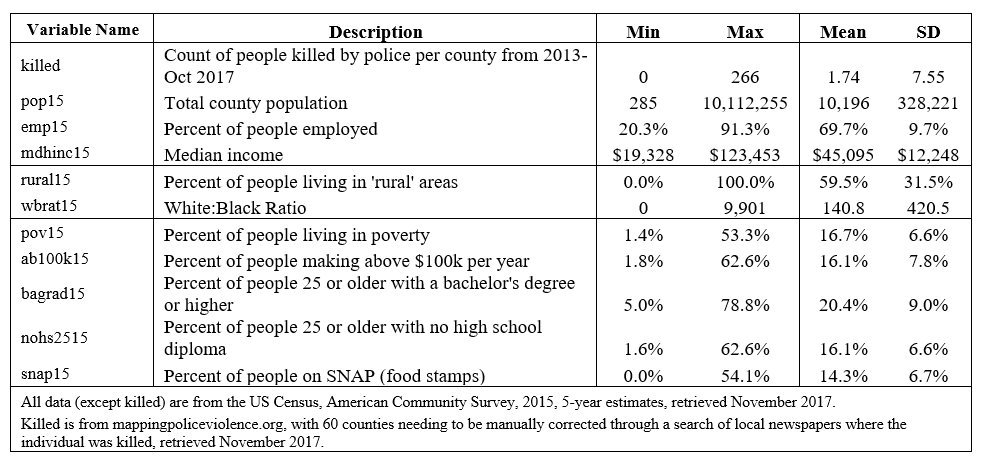
\includegraphics[width=1.0\textwidth]{images/table1.jpg}
\caption{All variables used in this study.}
\end{table}

The only race variable in this study is a ratio of White:Black population per county.  The Census uses self-identification of the individuals to label race.  Individuals can self-identify as multiple race and ethnic groups.  In this case, only those individuals listing a single race, White or Black, were counted, and a ratio was calculated.  The geography-type variable represents whether a person lives in a rural or urban area.  The census defines {\em urban} as any place with at least 2,500 people, and {\em rural} as everyplace else.  This variable is a percent of the county population who does not live in an urban area.  The two education variables only count those residents who are over 25 years of age, either who have a bachelor's degree or higher, or who do not have a  high-school diploma.  

There are five economic-related variables.  The first, percent of people employed compared to the county population, is taken only from those 20-64 years old.  The second measures the median income per county.  Income can be measured in several different ways, and while mean is a common measure of central tendency, it is often skewed up by high incomes, since low incomes are limited to zero.  Because of this, median income is typically used.  Two variables measure income deficits--the percent of people who have qualified for SNAP (food stamps), and the percent of people living below poverty.  The latter relies on the definition of poverty provided by the Office of Management and Budget, which varies this designation based on size and composition of the family.  The fifth measure is the percent of the population living above \$100,000  per year. The Census lists the median U.S. income at almost \$60,000 per year, and provides the \$100k data as a measure of a high-income county.

In addition to demographic and economic data, the Census Bureau provides a significant amount of geospatial information.  Through their TIGER products (Topologically Integrated Geographic Encoding and Referencing), they provide a web site where the public can download shapefiles at many different levels that are published each year, and can be connected to the rest of their data. \cite{tiger} For this study, county-level data was used, since it was the smallest administrative unit for which all of the data was available.  While accurate state-level data was available, it did not seem fine-grained enough to provide a sufficient analysis.  Smaller administrative levels, like census-tract, and even block-level shapefiles are available, and there is annual census data that can be mapped onto those levels.  While  some ACS variables are available at these small units, they typically only cover a random selection, and can have high error rates.  County-level data is the smallest administrative unit for which every county in the U.S. can be measured in the five-year estimates file.  The shapefile used for this study is the 2015 county-level data for the entire United States, and was downloaded from the Census TIGER site (November, 2017). \cite{tiger}  However, not all places available on the shapefile have data through the ACS.  For example, several of the smaller island territories are not included in the ACS survey, so those are excluded in the map, as well as the regression analysis.  While the latter includes Alaska and Hawaii, for ease of viewing the county-level data, those states are not included on the map (Figure 1).


\section{Methods}

There are multiple ways to attempt to understand police killings of citizens.  One way is by visualizing data of the events.  Another is by creating statistical models that relate the killings to predictor variables, such as in a regression equation.  Open source software is available for both of these approaches.

Quantum GIS (QGIS) is open source software that facilitates the visualization of spatial information, and is useful for tasks such as mapping, and seeing how data are related in geographic ways. \cite{qgis} For this project, QGIS 2.18.8 was used to process the Census TIGER shapefile (shp) that contained all of the United States counties.  When downloading files from the TIGER site, several other files come with the shp file, one of which is a database file (dbf) that contains information about each place identified in the shapefile.  For example, land and water mass frequently come with the dbf, along with geocodes and names that identify specific locations. 

In this case, since it is a county-level datafile, the first entry in the dbf is Cuming County, Nebraska, with Nebraska geocoded as state \#31, and Cuming County geocoded as county \#039.  All 3142 counties in the dbf file have these coded identifiers that match spreadsheets of demographic and employment data that can be downloaded from the Census Bureau, such as the ACS data.  Since the geocodes are identical, this data and the shapefiles can be easily integrated.  Integrating other types of data, such as the police killings data from MPV, requires a diffent approach.  In this case, since MPV provided both the county and state names where the deaths occurred, merging these into one string, such as "CumingNE", and doing the same with the TIGER shapefile data, the two files can be joined.  For Figure 1, which shows the rates of killings by police at the county-level, a ratio was calculated in QGIS--the count of those killed in each county divided by the total population of that county.  With the creation of this new variable, it can be mapped in QGIS as a {\em graduated symbol} with a prespecified color scheme. 

\begin{figure}
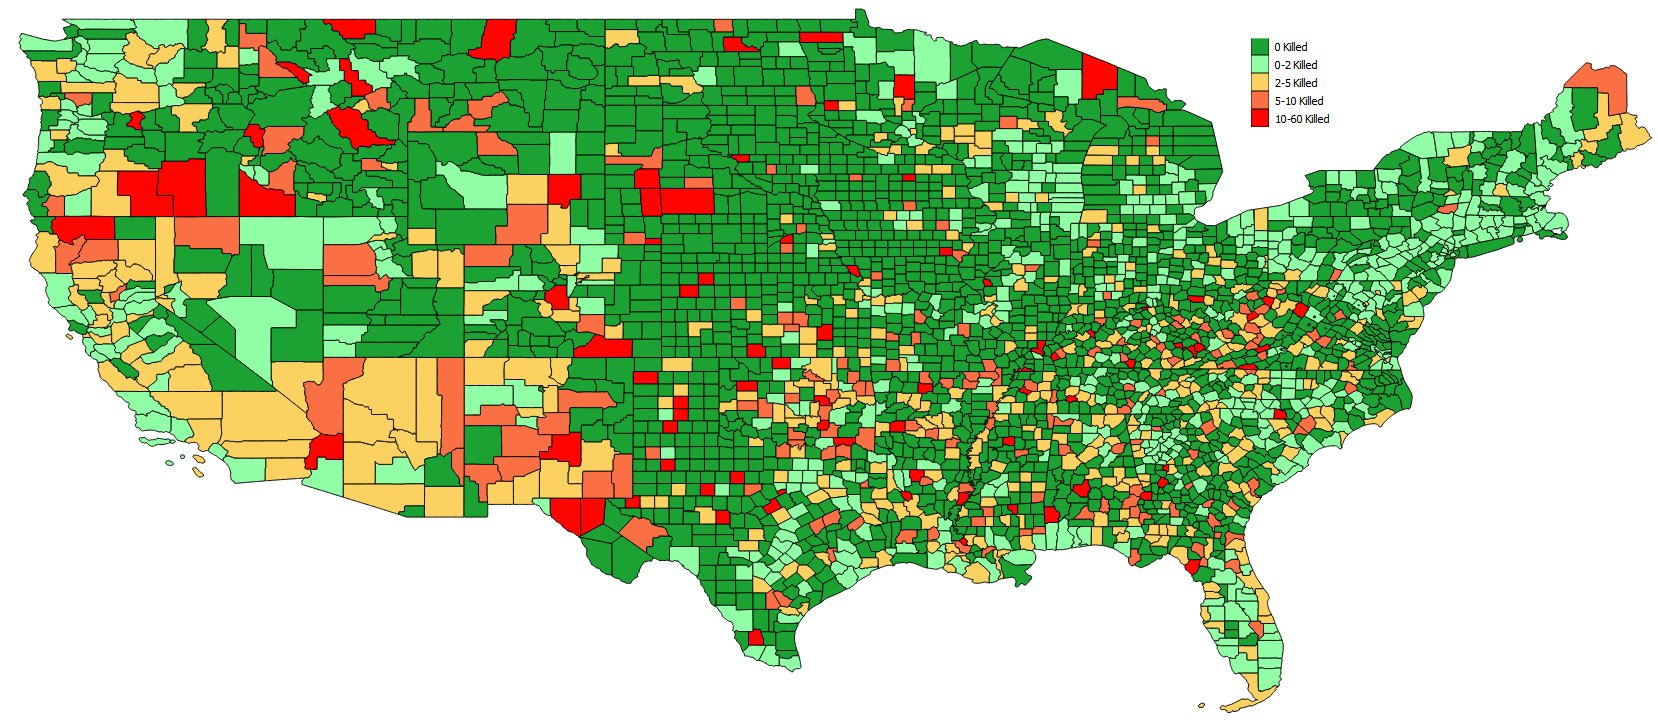
\includegraphics[width=1.0\textwidth]{images/figure1.jpg}
\caption{U.S. county-level map of residents killed by police, 2013-Oct 2017.  Data from Census and mappingpoliceviolence.org}
\end{figure}

This process can be automated with Python, a programming language useful for big data analysis. \cite{python}  QGIS has integrated Python into its software by including a Python Console for direct use, and an extensive instruction manual is available online through the QGIS web site. \cite{pyqgis}  For the map in Figure 1, a Python script was created that downloads a zipped file containing the TIGER shapefile for the US counties, and all of the census data that had previously been integrated into the dbf file. The script and data are available on the author's github course site. \cite{townsley} The zipped shapefile is available on the author's Indiana University Box account. \cite{townsley2} The Python program unzips the file, deletes all parts of the map except for the contiguous United States (all but 48 states), then applies a graduated color scheme to the killed/population ratio variable.

Regression analysis and graphs can also be accomplished through open source software, R, an environment for statistical analysis and graphics. \cite{r}  In addition to the base R package, which is command line only, other packages are available as an overlay to incorporate GUI features, such as RStudio. \cite{rstudio}  This analysis was done with R 3.4.1, using RStudio 1.0.153.  Instead of Python, R has its own scripting language.  The R-script for the following procedures and data are available on the author's github course site. \cite{townsley}

Creating a statistical model is a way to understand how variables are related to each other.  Regression analysis is a common way to model such relationships.  While more typically used with a continuous dependent variable, regression can also be used to model count variables.  In this case, the number of people killed by police is a count variable, and all of the predictor variables are continuous.  Modelling continuous dependent variables presumes a Gaussian distribution, but count variables often do not meet this assumption. \cite{fox15}  

Poisson and negative binomial distributions are typically better suited for count data. \cite{beaujean16}  These models often have a mass at zero, i.e., a very large number of zeros in the data. \cite{farewell17} In some cases, these zeros are structural, and in some cases the are {\em inaccessible}.  In the latter case, those zeros are assumed to be caused by a separate process than the process generating the rest of the values, the structural cause. \cite{neelon16}  Inaccessibility zeros are considered excessive, and a two-part, zero-inflated model would be a good option.  Zero-inflated Poisson, and zero-inflated negative binomial models are available in R.  A histogram of the dependent variable, and a plot of the dependent variable against the county population, are shown in Figure 2, with both graphs created in R.

\begin{figure}
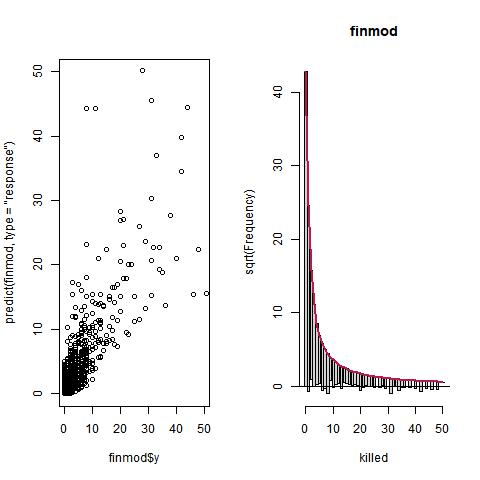
\includegraphics[width=1.0\textwidth]{images/figure2.jpg}
\caption{Left: Histogram of the number of county residents killed by police.  This histogram shows a maximum of eight per county killed by police, while the actual maximum is 266.  However, there are only 120 observations where this value is above 8.  This view gives a better depiction of the data.  Right: Scatter plot of the total county population versus the total killed by police in that county.  The red line is a regression prediction line for these two variables.}
\end{figure}

However, in the case of police killings data, a zero-inflated model is not theoretically sound.  Such models presume that there are a group of 'zero count' observations that are zero because it is impossible for that member to not be zero.  For example, if there were no police in a given county, then there could be no police killings in that county.  A health care example, is that if you were counting people in a given county who accessed health care services, and there was a group of people who lacked access to health care, they would be counted as zeros not because they did not need health care, but because they could not access it.  \cite{neelon16} Tetzlaff puts it another way, when explaining the choice not to use a zero-inflated model to analyze county-level child homicides: since every child has a chance of being killed (although fortunately most are not), a zero-inflated model would not be appropriate. \cite{tetzlaff13}  In other words, since there are no children for whom it is impossible to not become a homicide count, a zero-inflated model is theoretically unsound.

Other possible models are available for data with a mass at zero, for example, a two-part hurdle model.  However this approach would also be inappropriate because of hurdle assumptions.  For example, it presumes that all cases for whom becoming a count is possible, it will become a count--in other words, if criteria are met, then the subject would always move from a zero to a count. \cite{moore04}  Tobit models are often used with continuous data and a mass at zero.  But a Tobit zero is assumed to be possible censored data, such that it is some value other than an actual zero.  In this case, where a count of police killings is the dependent variable, a zero represents a true zero, not a possible censored zero, so a Tobit model is also likely not a good choice. \cite{neelon16}  

One of the assumptions of a Poisson distribution is that the mean and dispersion are equivalent. \cite{fox15}  A model with a variance greater than the mean is considered over-dispersed, which implies it is a better candidate for a negative binomial regression approach.  As can be seen in Table 1, the mean of the count killed by police is 1.74, and the variance is 57.0 (square of standard deviation, 7.55).  This data is clearly over-dispersed, and a good candidate for negative binomial regression.

\section{Findings}
Three regression models were created: the full model, which includes all of ten independent variables; the partial model, which includes only five independent variables; and the final model, which includes the best three predictors.  The coefficients and p-values of these models can be found in Table 2, along with a  number of diagnostic criteria.  From the full model, all of the non-significant variables were removed to generate the partial model.  From the partial model, both variables that were less than p=0.10 were removed from the model, leaving three predictor variables, all of which were significant to p$\leq$0.001.  By all measures, the three models have very similar model fit and diagnostic criteria (AIC, R-square, correlation between predicted and observed, RMSE, predicted mean of outcome variable, etc.).  The variance inflation factor was checked for each, and while significant problems were detected for the full model (max VIF=34.5), those problems were eliminated in both of the smaller models.  The final model seems like the best candidate since it is the simplest, with only three predictor variables, and having equivalent goodness-of-fit values as the more complex models. 

\begin{table}
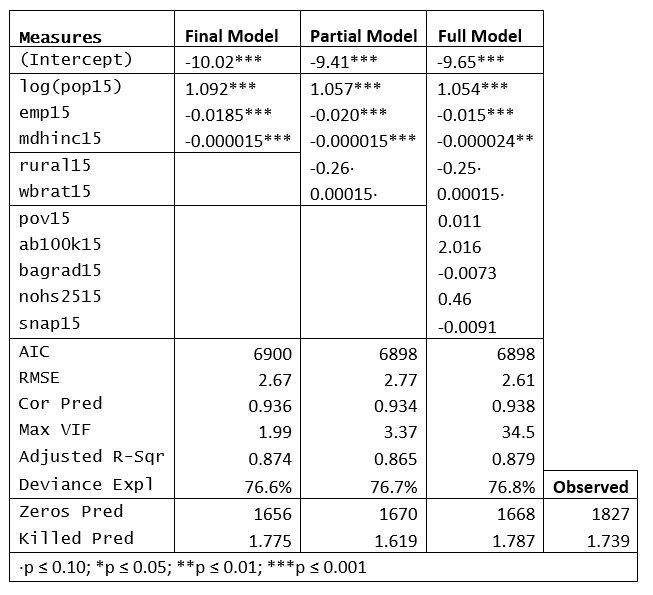
\includegraphics[width=1.0\textwidth]{images/table2.jpg}
\caption{Regression and diagnostic results from all three models.  "Zeros Pred" are the number of counties where no person is predicted to be killed by police, calculated not at exact zero, but any value less than 0.5.  "Killed Pred" is the mean number of predicted people killed by police in each county.}
\end{table}

The final regression model indicates a strong relationship between the dependent variable, the count of people killed by police by county, and the three predictor variables, population of the county, employment rates in that county, and county median income.  The coefficients indicate both strength and direction of the relationship, and can be used to create a prediction equation. \\ 

Killed by Police = -10.01 + 1.092 * log(Population) - 0.0185 * Employment Rate - 0.000015 * Median Income\\

This implies that the higher the county population, the higher the risk of being killed by police, the higher the employment rate in the county, the lower the risk of being killed by police, and the higher the county median income, the lower the risk of being killed by police.  According to output from the R regression analysis, this three-variable model explains 76.6\% of the variance of the dependent variable, and the predicted vs observed killings by police have a correlation of 0.936.  The mean predicted killings are 1.775 per county, while the observed killings were 1.739.  This model predicts 1656 counties will have approximately zero killings (less than 0.5), while the actual number of counties with no killings was 1827.

Figures 3 shows two R graphs supporting the conclusion that the final model is a good fit.  The left plot of predicted versus observed killings by police per county, with the red regression line of just these two variables, shows the strong relationship between them.  The rootogram on the right shows that few bins of predicted outcomes are significantly divergent from the observed values.  A rootogram is interpreted by the {\cm hanging} bars--bars hanging above the zero-line are over-fit, while bars hanging below the line are under-fit. \cite{rootogram}  The closeness of the bars to the zero-line indicate a relatively good fit.

\begin{figure}
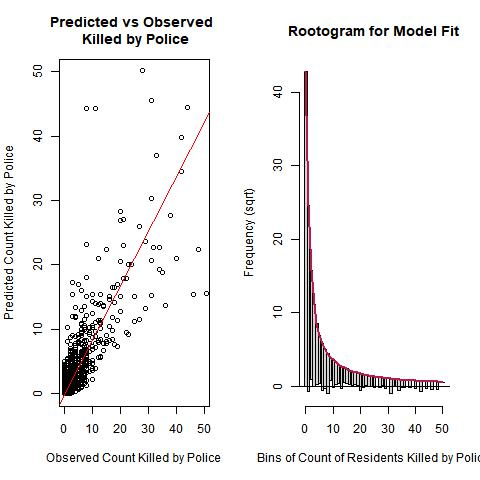
\includegraphics[width=1.0\textwidth]{images/figure3.jpg}
\caption{Left: Scatter plot of predicted versus observed counts of residents killed by police per county. Right: Rootogram--fit of the final regression model: negative binomial with three independent variables (log of population, employment and median income).  The red line can be interpreted as the observed values.  Bars that are hanging below the zero-line are under-fit for that bin, and those above the line are over-fit for that bin.}
\end{figure}

In addition to goodness of fit, regression also requires that residuals meet basic assumptions.  Figure 4 shows several standard diagnostic plots indicating that these assumptions are met.  The residuals versus fitted values plot is interpreted as being problematic if a pattern emerges from the residuals, either above or below the zero-line.  In this case, no pattern is apparent--the residuals seem equally and randomly scattered above and below the line.  Similarly, the plot of residuals versus index shows a similar result, indicating the regression residuals assumption is met.  Finally, the bottom two plots, more residuals plots, show the same.  For example, the {\em Normal Q-Q Plot} would indicate a problem if a significant number of dots were straying from the main central line--in this case they are almost all on the line. \cite{hocking}

\begin{figure}
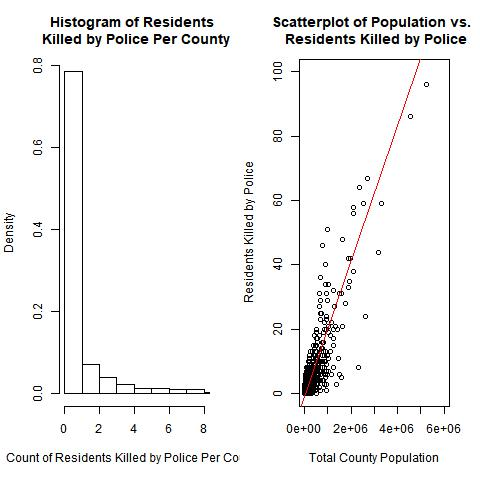
\includegraphics[width=1.0\textwidth]{images/figure4.jpg}
\caption{Regression diagnostics plots for the final model with three independent variables: population (log), employment and median income. Top: Residuals versus fitted and residuals versus index.  Bottom: Quantile residuals and QQ Plot of residuals. }
\end{figure}


\section{Conclusion}
\bibliographystyle{ACM-Reference-Format}
\bibliography{report} 

\end{document}
